\newcommand{\tachyon}{\textsc{Tachyon}\xspace}
\chapter{\tachyon: Tandem Execution for Efficient Live Patch Testing}
\label{chap:tachyon}
\newcommand{\allsystemcallreplay}{patil:2010,guo:2008}
\newcommand{\allinstructionlevelreplay}{patil:2010,gdb,undodb}
\newcommand{\allvmreplay}{retrace,simics,vmware-replay}
\newcommand{\patched}{P}
\newcommand{\unpatched}{P'}
\newcommand{\tuple}[3]{\langle #1, #2, #3 \rangle}
\newcommand{\size}[1]{|#1|}
\newcommand{\len}[1]{\mathsf{len}(#1)}
\newcommand{\seqlen}[1]{\mathsf{seqlen}(#1)}
\newcommand{\impl}{\rightarrow}
\newcommand{\etal}{et al.\ }

In order to show that Holmes can be used in practice, we implement a concrete system with it.
We chose to focus on the problem of use-after-free, as it is a little-explored area for static binary analysis.
We used Holmes here to link together control flow analysis, alias analysis, string recovery, and general function loading in order to build a working use-after-free engine.

% Use after free bugs are common
There were 238 use-after-free (UaF) vulnerability disclosures (CWE-416) issued in 2017 alone, with 36.2\% given a critical security
rating.
% From cvedetails.com, mitre doesn't seem to issue CVE/CWE associations.
Use-after-free bugs happen when a pointer has been freed and the memory pointed to subsequently written to or read from.
Use-after-free bugs can lead to DoS, control flow hijack, and information leaks.

Despite the number of CVEs, few tools exist that can automatically and statically detect such bugs in off-the-shelf \emph{binary} code.
However, there are tools for finding such bugs in \emph{source} code.
Requiring source code limits the applicability of these techniques to developers with full source access.

In this chapter, we focus on the question
``Can we use \sysname\ to bridge the gap between analysis for UaF bugs in source code versus compiled code?''
In particular, previous work has been unable to apply source code techniques to compiled code.
Can we adapt such techniques to be effective even without source?

At a high level, UaF bugs require reasoning about memory allocation and memory aliasing.
Source code techniques are more plentiful due to the rich and mature research area of alias, points-to, and similar schemes for reasoning about memory over the lifetime of a program.
In comparison, at the binary level the primary approach for reasoning about memory is Value Set Analysis~\cite{vsa}, which is less mature and has several limitations in practice such as inability to reason about all arithmetic operations (e.g., bit-shifts and division) and the fact it may not terminate without ad-hoc widening in the presence of loops.
For example, GUEB~\cite{gueb} was proposed to detect UaF bugs using VSA, but is handicapped by disallowing cyclic paths to allow rapid termination of VSA.

We present a new binary-level static analysis approach for detecting UaF bugs in executable programs.
One of the main technical challenges we address is showing how to adapt source-code memory alias analysis to compiled code, where previous work has instead created all-new binary-only approaches to alias
analysis like VSA.
We experiment with two classes of analysis: flow insensitive alias analysis via a Steensgaard-type~\cite{steensgaard-alias} algorithm, and  flow-sensitive alias analysis using a data flow approach adapted from Andersen~\cite{andersen} style analysis with added rules to handle binary-specific details such as calling conventions and computed addresses.
We also add context-sensitivity by allowing the analysis to reason about the call-stack discipline followed by executable code, and a type of field sensitivity appropriate for direct pointer arithmetic without type information.
To the best of our knowledge, very little work has been done in applying the literature in source alias analysis to compiled code, and no previous work has shown how to then use such techniques to find UaF bugs statically in compiled code.

We have built a tool called \aliasname\ that uses \sysname\ to drive the different levels and co-dependencies in binary analysis, alias analysis, and UaF detection.
Taking this approach allows us to have an end-to-end reasoning chain from input binary to why this particular candidate use-after-free could not be disproven with a given sensitivity.

We evaluated \aliasname\ over 7 real CVEs and the Juliet test suite released by IARPA for purposes of verifying our detection capabilities and measuring false positives in the face of bugs.
Additionally, we measured false positive rates against a background of expected-good binaries (we assume no true positives): a random sampling from the \texttt{\$PATH} of a default Ubuntu installation.

\aliasname\ is available at \url{https://github.com/maurer/marduk}.

\section{Design of \tachyon}



\subsection{Overview of \tachyon and Challenges}

\begin{figure}
  \centering
  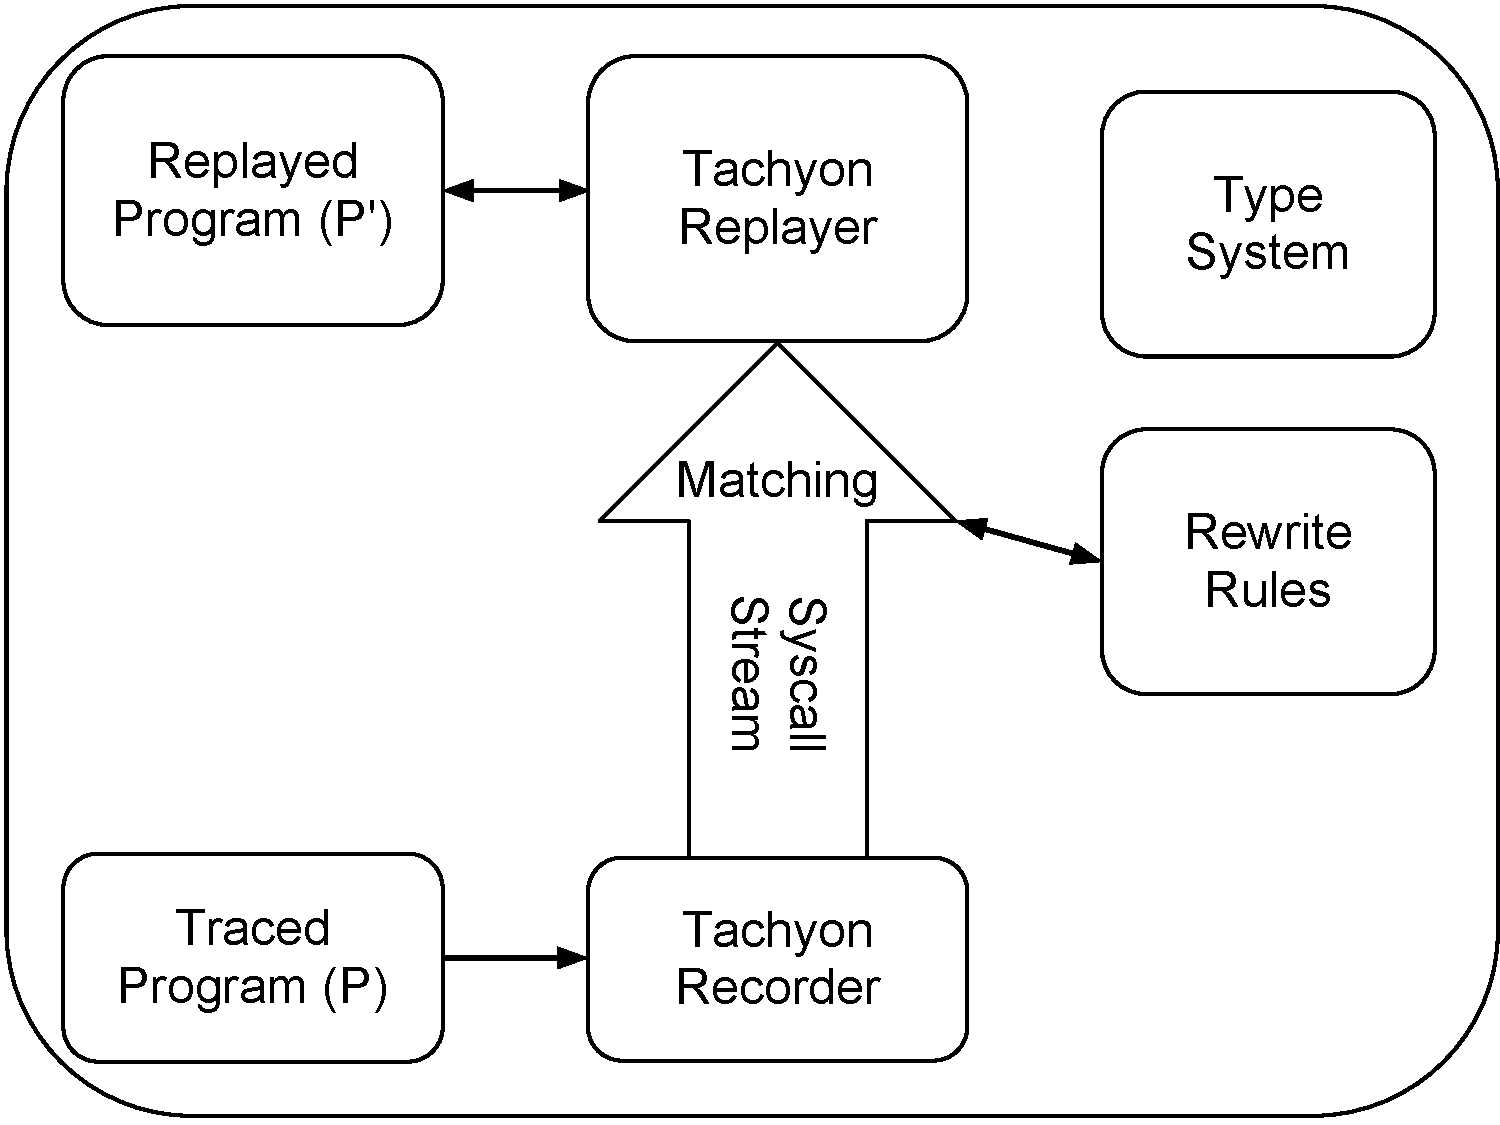
\includegraphics[scale=0.5]{tachyon/TachyonDiagram.pdf}
  \caption{Tachyon System Overview}
  \label{tach:fig:system}
\end{figure}

The overall architecture of \tachyon is shown in
Figure~\ref{tach:fig:system}.
We will refer to the program running
live  as $\patched$ (e.g., the patched program) and the program running
in-tandem with simulated syscalls as $\unpatched$ (e.g., the unpatched
program).  \tachyon is a user-land program that utilizes the Linux
ptrace facility to interpose on syscalls issued by $\patched$ and
$\unpatched$.  Like replay schemes, \tachyon has a recorder and a
replay module. The recorder records the stream of system calls
issued by $\patched$ and outputs a stream of tuples
$\tuple{C}{\vec{I}}{\vec{O}}$ where $C$ is the system call number,
$\vec{I}$ is a list of inputs to the system call, and $\vec{O}$ is a
list of outputs.  The replay module interposes on $\unpatched$, and
for each syscall $C$ with arguments $\vec{I}$ made by $\unpatched$,
simulates the OS by returning $\vec{O}$.

\begin{lstlisting}[float,caption={Example patch},label={tach:lst:example}]
-int fd = open("/tmp/fileA", O_RDONLY);
+int fd = open("/tmp/fileB", O_RDWR);
-int *storage = malloc(...);
-/* ... Do some processing with storage..  */
+fstat(fd, statBuf);
 char* incoming = malloc(chunksize);
 ssize_t size = read(fd, incoming, chunksize);
 if (size != -1)
   write(fdOut, incoming, size);
\end{lstlisting}

Consider the example shown in Listing~\ref{tach:lst:example}, with the
patch difference being displayed in diff style with full context. The first
edit changes the file opened from \texttt{/tmp/fileA} to
\texttt{/tmp/fileB}. The next few edits remove an unneeded call to
{\tt malloc}, and add {\tt fstat}.  The rest of the program is the
same. Note that since a {\tt malloc} call was removed, the returned
memory chunk for {\tt incoming} will be at a different address, even
on systems with a deterministic memory layout.  Overall, this patch
example illustrates three challenges: patches may change arguments to
system calls, may change system calls issued, may change memory
allocation patterns, and any of these changes may have effects on subsequent
execution.

% Essentially, we see here an earlier bit of processing which used an allocation
% was removed, along with an unneeded \texttt{fstat}. The call to \texttt{write}
% emphasizes the challenge of isolation for tandem execution, as a bad program
% would clobber the output of the good program. The change in allocations between
% the two moves the memory layout around, making memory diffing techniques
% ineffective for recording effects, emphasizing the second challenge. Finally,
% the spurious \texttt{fstat} which is dropped in the patch should be accepted,
% showing the need for a system call stream rewriting.


The above challenges motivate three main requirements of live patch
testing as distinguished from a normal replay system. First, instead
of offline replay, a live patch testing solution should be
\emph{online} where $\patched$ produces the syscall stream that
$\unpatched$ should consume.  Second, a live patch tester should not
depend upon pointers because absolute memory addresses may change
between runs. For example, $\unpatched$ and $\patched$ may issue
calls to {\tt malloc} for different amounts or ASLR may be enabled.
Either case prevents patch testing. As a result, we cannot determine
$\vec{O}$ by simply diffing the memory state
before and after a syscall, as in previous syscall replay
schemes~\cite{\allsystemcallreplay}.  Additionally, memory diffing
does not allow us to determine the inputs $\vec{I}$ to system
calls. As a good live patch tester should verify the inputs as well,
we need some way to extract all inputs of a system call. Without a
semantic model, we will be unable to both locate all the relevant
components of the input, and to avoid capturing irrelevant components.
Thus, we need a semantic model of the inputs. Third, since a patch
may remove or add system calls, the live patch testing scheme should
allow for the syscall stream to be rewritten during replay. This can be accounted for by allowing
rewriting of the tuple stream $\tuple{C}{\vec{I}}{\vec{O}}$.  


\subsection{System Calls and Side-Effects}

\tachyon needs to determine what the semantic inputs and outputs
to a syscall are in order to record and replay them.  Specifically, it needs to (1) determine the types of
arguments to a syscall, (2) differentiate input from
output, and (3) pointers from the pointed-to data. While existing C
syscall prototypes are sufficient  for (1), they do not provide enough
information for (2) and (3). Consider the
\texttt{read} syscall declaration:
\begin{lstlisting}
ssize_t read(int fd, void *buf, size_t count);
\end{lstlisting}

This C declaration misses crucial information.  First, it
gives no clue how the void pointer buf works. How big is it? Is it
null-terminated? Are the contents relevant before the call, after, or
both? We need to answer all these questions in order to copy the
appropriate semantic data.  We can see that even the assertion that a
pointer points at some data before or after the system call is not the
case, as with \texttt{sbrk} (pointer points at the end of your address space)
 and \texttt{mmap} (one pointer is only a suggestion). {\tt read} is one of the
simple cases; several syscalls have complicated dependencies between
input and output parameters, as will be discussed later in~\S\ref{tach:sec:types}.

\tachyon addresses the challenges associated with understanding the
syscall semantics by adding type annotations, as described in~\S\ref{tach:sec:types}. The \tachyon 
annotation language is a light-weight dependent type system that says
how to parse the inputs and arguments into semantic data at runtime.
These type annotations only need to be written once per system call,
and are portable across systems with the same syscall signatures.

\subsection{Syscall Stream Rewriting}

%\edissue{Maurer: Done. Honestly, I liked cURL better, but I understand trying to have a single example for the section.}

Many patches also change the sequence of syscalls made in addition to
the actual parameters.  Consider Listing~\ref{tach:lst:example}.  The
system call stream when executing the patched program is $\langle ...,
{\tt open}, {\tt fstat}, {\tt read}, {\tt write}, ...\rangle$.
However, the call after {\tt open}  in the unpatched program is {\tt
  read}, not {\tt fstat}.  

%Thus, the two programs have semantically
%different behavior, which we will report as a deviation.



New patched versions often have new system call patterns that cause
the program to behave differently at an IO level. It is not possible
to tell whether a particular change in system call patterns is valid
without a human to validate it. For example, if it turns out the
above code is just shifting a few things around and adding a new
inconsequential call to \texttt{fstat}, then the user may want to
ignore the deviation.  However, the \texttt{fstat} may have been
inserted for security, and a deviation may indicate an attack.  When
opening files in \texttt{/tmp/} a common security practice is to
then call \texttt{fstat} to obtain the user ID and group ID of the
file to make sure they are correct in order to detect race
conditions. \tachyon should report the deviation and halt execution in
such instances. 

Although we cannot automatically decide which deviations matter,
\tachyon does \emph{automate finding deviations}, as well as provide a
mechanism to ignore such deviations when found to continue testing.
The rewriting engine relies upon rules that are created for each
patched program that detail how to handle semantic differences. For
example, if a system administrator decides the above deviation is
inconsequential a rule can be written to ignore the {\tt fstat} call.
Alternatively, patch creators could write such rules and distribute
them with their patches to aid testing.

\subsection{Road Map}
In the rest of this chapter, we first describe the \tachyon type system in detail. We
then discuss how \tachyon rewrites system calls, as well as some
common rules we have found in patches we have tested. We next describe
our implementation and evaluation. We finally discuss several
applications of \tachyon outside automated patch testing.


%%% Local Variables: 
%%% mode: latex
%%% TeX-master: "paper"
%%% End: 

\section{System Call Types}
\label{tach:sec:types}

The C function declarations for syscalls do not describe all
side-effects. \tachyon proposes an extension to the C type
declarations to encode all semantic information necessary to record
which parameters are inputs, which are outputs, and how to identify
all bytes for each parameter. While this problem has been attacked before~\cite{guo:2008},
our particular needs are different due to the binary only-nature of our
approach, as we discuss in \S~\ref{tach:sec:related}.

The \tachyon type system takes advantage of the
user-space/kernel-space barrier for interposition. The barrier
provides a clean separation that can be monitored without
requiring source to the program. In addition, the barrier allows
\tachyon to not monitor internal kernel state. The reason is that the only
way $\unpatched$ and $\patched$ can interact with the underlying
system is via \tachyon, and \tachyon's mechanism ensures that both
programs see an identical state.  This is a vital complexity
reduction.

\tachyon uses a limited form of lightweight dependent types (types
which depend on values). Our lightweight use avoids pitfalls such as
undecidability normally associated with dependent types. In the rest
of this section, we first provide an intuition on the issues and how
dependent types are used, and then describe the full system.


\subsection{Intuition}

A basic approach for recording syscalls is to decorate C types with
information about which parameters should be treated as inputs,
outputs, or both.  We call such annotations the IO class for each
parameter.  In order to specify how to copy output parameters, we also
need to know the size of their values.  The size information is needed
because we need to copy all output bytes from {\tt buf} in the
monitored program $\patched$ to the address space of $\unpatched$.
For example, we could imagine annotating the {\tt read} call as:
\begin{lstlisting}
ssize_t read(int fd, void output* buf{ret}, size_t count);
\end{lstlisting}
The parameter {\tt buf} has been annotated as an output parameter,
thus should be copied and replayed to $\unpatched$.  The annotation
also specifies that {\tt ret} bytes should be copied, where {\tt ret}
is the return value.


Unfortunately, such simple annotations are insufficient with many data
structures, such as vectors. A prime example of a difficult system
call is \texttt{readv}, which provides vectored reads of a file
descriptor. Its C type declaration is:
\begin{lstlisting}
ssize_t readv(int fd, const struct iovec *iov, int iovcnt);
struct iovec {
  void  *iov_base; /* Starting address */
  size_t iov_len; /* Num bytes in iov_base */
};
\end{lstlisting}
The main issue demonstrated is that a complete description of the IO behavior of
parameters may refer to other parameters.  The {\tt iov\_base} length
is determined by {\tt iov\_len}, and the total number of {\tt iov}
items is given by {\tt iovcnt}.  \texttt{readv} is not alone: it has
many friends such as \texttt{writev}, \texttt{preadv}, and
\texttt{pwritev}. In order to handle such cases, we need a type system
that allows us to express \emph{relationships} between parameter values.

% Suddenly, it is less clear exactly how to encode this, and this system
% call is not alone, there are a number of others like it, though it
% and its friends 
% are somewhat unique in that they exercise three cases not addressed by the
% previous system (pointers not in an argument, sizes not in an argument,
% and variable numbers of pointers). In particular, we are now on to a more
% dependent type system, as the exact type is dependent upon a function of the
% values, e.g., the size of the buffer pointed at by \texttt{iov\_base} is
% determined by the lenth next to it.


\begin{figure}
	\begin{center}
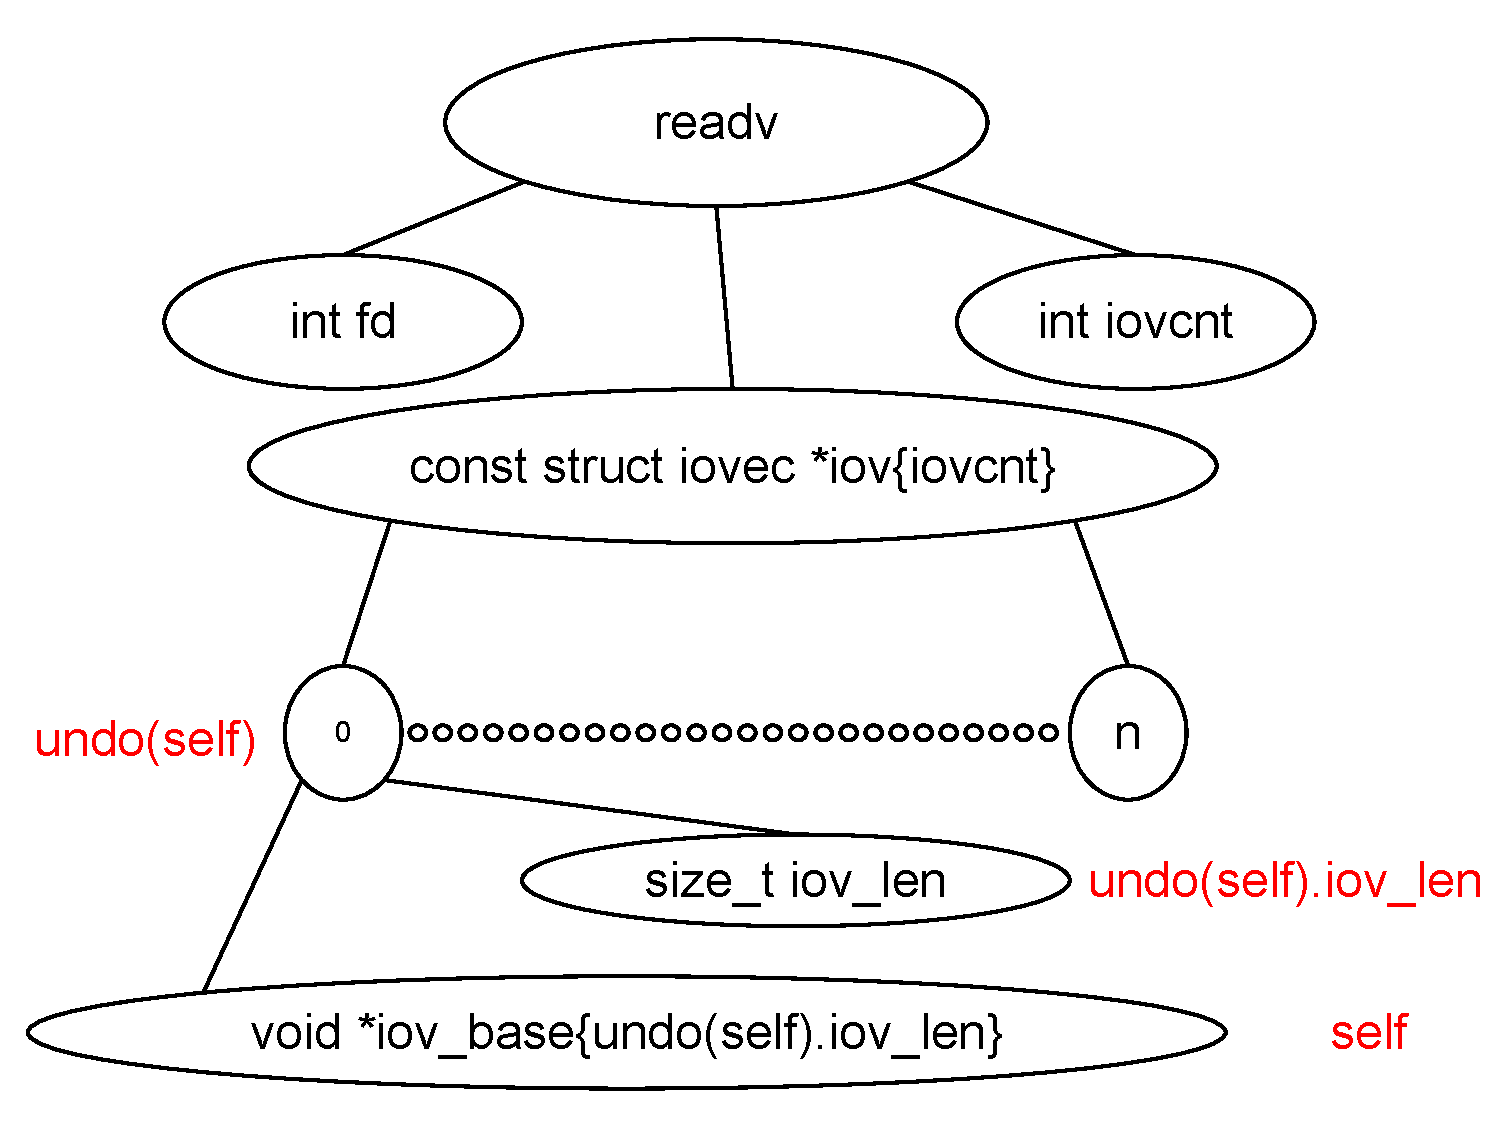
\includegraphics[scale=0.4]{tachyon/LookupDiagram.pdf}
	\end{center}
\caption{A lookup in action}
\label{tach:fig:lookup}
\end{figure}


\tachyon uses lightweight dependent types that can express
relationships between the value of one parameter and the value of
another.  We view types as a tree, and use dependent types to walk the
tree to determine a value.  


The types allow us to walk from the top of the tree, or from the
current parameter.  In \tachyon, we specify {\tt readv} as:
\begin{lstlisting}
ssize_t readv(int fd, const struct inputoutput iovecin *iov{iovcnt}, int iovcnt);
struct iovecin {
  void input *iov_base{undo(self).iov_len};
  size_t iov_len;
}
\end{lstlisting}
We now call the struct \texttt{iovecin}, because while both
\texttt{readv} and \texttt{writev} take an \texttt{iovec}, they are
used differently, and so are assigned differing types (specifically,
in one case the buffers inside are output, while in the other they
are input).  The only new annotations compared to before are
\texttt{undo} and \texttt{self}, which are used to walk the type
tree to reference other fields. The semantic meaning is that
\texttt{iov\_base} is \texttt{iov\_len} bytes.  \texttt{self} refers
to the location at which the current value is being read from.
\texttt{undo} simply says to step back along whatever indexing step
was done to get there.  In this case, this means that \texttt{self}
represents the tree traversal up through that instance of
\texttt{iov\_base}. The ``undo'' brings us up a level, to be looking
at the struct. Then, we index the struct to \texttt{iov\_len} and are
done.  Figure~\ref{tach:fig:lookup} graphically shows the type tree for
\texttt{readv} and how the syntax expresses fields in the tree.

% This is useful as a point of
%reference so that structs can have self contained types, allowing for
%reuse across functions (and can exist in arrays like the one we have
%here).


\subsection{The Tachyon Type System}
The full \tachyon dependent type system is shown in
Figure~\ref{tach:fig:annotations}, and is taken directly from the \tachyon
source code in Haskell.  The language is similar to BNF, where
non-terminals are to the left of the equal sign, and brackets denote
a list (e.g., [A] is a list with elements of type A).


\begin{figure}
\lstset{language=Haskell}
\begin{lstlisting}
data SysSig = SysSig Type [Type]
data Type = Small Int
          | Struct [Type]
          | Ptr IOC Type Bound T
data T = NT | UT
data IOC = In | Out | InOut
data Bound = Const Int | Lookup Lookup
data Lookup = Ret | Arg Int | Index Int Lookup | Self | Undo Lookup
\end{lstlisting}
\caption{The \tachyon annotation language}
\label{tach:fig:annotations}
\end{figure}

In \tachyon's language, IOC represents an IO class, that is, whether
the pointer is input, output, or both.  T represents some form of
termination, to allow us to include null-terminated data. NT is for
null-terminated data; UT is for unterminated data. If a pointer is
null-terminated, reading will cease when a 0 is hit, if this happens prior
to the end of the buffer. The index operation is used on both arrays
and structs, where the $i$'th index refers to the $i$'th field
(counting from 0).

The types available are
\begin{itemize}
\item Small - These correspond to basic integer C types, like
  \texttt{char} or \texttt{long}, and indicate values that should not
  be treated as pointers. The type parameter is the number of bytes of
  the type, e.g., Small(1) is a 1-byte value corresponding to a {\tt
    char}.

\item Struct - an aggregate of other types. Note that previous replay
  work treated such types as raw buffers because they could determine
  size by simply diffing memory before and after a syscall.  In live
  replay, we explicitly lay out all fields because the underlying
  types may yield further information.

\item Ptr - a pointer  annotated with an IO class, the type of
  element it is pointing to, a way to tell how many elements it points
  to, and whether or not it respects a null termination convention.
\end{itemize}

We introduce the concept
of a ``lookup''. This is just a series of steps that can be performed
from either the arguments of a function in the case of an input or
in/out class pointer, or the arguments and return value in the case of
an output pointer, to arrive at a memory location or register. This is
demonstrated in Figure~\ref{tach:fig:lookup}. The Ret and Arg
constructs for a lookup are used to allow us to reference the return
value or various arguments in a system call, respectively.  This is
just the generalization of the tree walking described earlier.

Given this, the encoding of a bound as either a constant or a lookup
is rather natural. It is the use of this bound that makes us lightly
dependently typed---the type depends on the data in question.

Finally, we can build the fundamental structure all this is for---the
system signature.  A system signature, indicated by SysSig, is what is
assigned to each system call in order to allow the tracer to
record and play back its effects. The first parameter is the type of
the return value, and the second is a list of the types of its
arguments.

\paragraph{Type Checking \tachyon Declarations.}

The \tachyon types need only be written once for each system call,
and can be reused for any program.  However, since they are written
manually, we would like to prevent mistakes.  In order to achieve
this, \tachyon also provides type-checking to make sure the
annotations make sense. In particular, \tachyon checks:
\begin{enumerate}
\item Bounds are numbers, not pointers or something else.
\item Bounds use only information which is available for the IO class of the pointer (e.g., input class may not use the return value as a size).
\item Output pointers do not contain structure; they are raw data.
\item Types are potentially compatible with the original C type.
\end{enumerate}
These checks ensure annotations which are usable, self-consistent, and match
the C type. 


%%% Local Variables: 
%%% mode: latex
%%% TeX-master: "paper"
%%% End: 

\section{System Call Stream Deviation Detection and Rewriting}
\label{tach:sec:equiv}

Patches often add, delete, or modify  new system calls in the original
buggy program.  Our example in Listing~\ref{tach:lst:example} shows all
three cases.  When the streams of syscalls differ, then the two programs are
semantically different.  While this means we cannot automatically tell
if the differences are meaningful, we can (a) automatically detect
deviations and (b) rewrite deviations when informed by the user that
the semantic differences are permitted. The heart of detection and
rewriting is \tachyon's syscall stream matching and rewriting engine.

% When the syscalls change between$\patched$ and
% $\unpatched$, then 

% Since the patch introduces semantically different I/O, it is
% impossible to automatically decide whether the changes are
% inconsequential or not. However, we can (a) automatically
% \emph{detect} 

% Naively, you might expect that pre and post-patch programs will always
% issue the same set of system calls on normal inputs.
% Unfortunately, this is not the case.
% For example, if a program changes the size of the
% buffer in a bulk transfer from 1024 to 4096, this will
% cause a change in the system call stream (fewer read/write calls), while causing
% little or no change in the effects.

\subsection{Stream Matching}

\tachyon uses a rule-based system for rewriting
system call streams during execution, designed to be employed by a
user of the tracing software to explain to the system what behaviors
it should consider equivalent. The rules must consume a sequence of system calls by
$\patched$, and produce a corresponding set of system calls for $\unpatched$ to
make in order to allow for writing call results into $\unpatched$ and checking
that $\unpatched$ indeed matches the particular equivalence rule.

As we execute, we have two streams of tuples. \tachyon represents the
stream from $\patched$ as $\tuple{C_i}{\vec{I}_i}{\vec{O}_i}$, and the
stream from $\unpatched$ as $\tuple{C'_i}{\vec{I}'_i}{\vec{O}'_i}$.
The easy case is when the two programs are semantically equivalent by
issuing the same system calls, i.e., $\forall i: C_i = C'_i \land \vec{I}_i = \vec{I}'_i$.  In this case no rule is needed, and
\tachyon will send the corresponding $\vec{O}_i$ for each $\vec{I}_i$ to $\unpatched$.

Any time the syscall input arguments do not line up, \tachyon reports a
semantic deviation.  In order to permit some deviations, \tachyon
provides the ability to rewrite the system call stream.  The rewrite
engine takes in a set of rewriting rules $f$.  Each rewrite rule $f_k$
is a function which takes in $\tuple{C_i}{\vec{I}_i}{\vec{O}_i}$ and
$\langle C_i', \vec{I}'_i \rangle$. 
The rule uses pattern matching
to decide if it applies, and if so, returns a pair of equivalent syscall
streams to perform a substitution with.
After a
match, the stream continues to be consumed by the simulated program $\unpatched$. 

% In the simplest case, each sub-stream is of length 1, and so we
% get a deletion sub-stream that looks like
% $\tuple{C_i}{\vec{I}_i}{\vec{O}_i}$, and an insertion sub-stream that
% looks like $\tuple{C'_i}{\vec{I}'_i}{\vec{O}'_i}$, where $\vec{O}'_i$
% is generated by the function in question.

The overall mechanism can be used for:
\begin{itemize}
\item Determining roughly equivalent  syscalls, e.g., many small
  writes being patched to be one big rewrite.
\item Ignoring syscalls, e.g., the $\patched$ program issues a call
  that is not needed by $\unpatched$. 
\item Limited reordering, e.g., allowing for syscalls to be switched.
\end{itemize}


%\edissue{You suggested this section needed to be rewritten for clarity. Have these changes done the trick?}


\subsection{Rewriting Rules}

Each rewrite rule $f$ takes a system call (the one made by $\patched$)
and the input to a potential system call made by $\unpatched$, and
returns a substitution in the stream. The substitution is implemented
as a pair of lists, where the left list indicates the syscalls
consumed by the rule, and the right list indicates the corresponding
substitution produced by the rule.  The type signature for $f$ in
\tachyon is:
\[
\text{Syscall}  \impl \text{SysReq} \impl \text{Maybe ([Syscall],
  [Syscall])}
\]
\noindent where the ``$\text{Maybe}$'' indicates that the rule may also return that
no substitution was performed. 


The rewriting rules are pure functions, which means they have no
access to outside resources like the current syscall stream or
application state.  By being pure we ensure that rewrite rules can be
applied in any order.  In addition, it ensures that the rule engine
itself will not continually accumulate state, i.e., while individual
rewrites may take substantial space, the space used will remain
constant in the number of system calls which have gone through, which
is vital to an online system.


During execution, the matching engine maintains a queue of syscalls
executed by the live program $\patched$.  Suppose the queue contains
any syscall $x$ that is not \texttt{write}, but the simulated program
$\unpatched$ issues a \texttt{write} syscall.  The simplest rule is to
ignore the \texttt{write}.  This is accomplished by adding a
\texttt{write} to the queue before $x$.  When the matching engine
re-examines the queue, it will match the still-pending \texttt{write} to the
one in the queue, and not report a deviation.

In \tachyon, the rule is written as:
\lstset{language=Haskell}
\begin{lstlisting}
ignoreWrite :: Syscall
            -> SysReq
            -> Maybe ([Syscall], [Syscall])
ignoreWrite x (Write 2 buf sz) =
  Just ([x],
        [Syscall (Write 2 buf sz) sz, x])
ignoreWrite _ _ = Nothing
\end{lstlisting}

This rule fires when line 4 is matched. This occurs when $\patched$
issues a syscall $x$ that doesn't match $\unpatched$'s syscall
\texttt{write}. On line 5 the rule directs it to consume whatever is
on the stream at the moment, and replace it on line 6 with the stream
of \texttt{Write} followed by $x$. This can be thought of as
``faking'' the call for \texttt{Write} to the stream matcher so that
it does not report a deviation. On line
7, we catch the case where our conditions are not met, and
indicate we did not modify the stream.

The simple, no-look-behind method of replaying with this equivalence
is to replay the stream normally until a match fails. At this point,
the two syscalls that failed to match are fed into all rewrite rules,
and their replacement list for the original stream is checked. If
there is still more than one rewrite rule remaining, one is chosen
arbitrarily. In future work, checkpointing could be used here to allow
for the ability to rewind if the wrong replacement was chosen.  In
practice, the rules we tested have only yielded one matching rewrite.

%In this way, we can safely describe a looser form of equivalence that
%still allows for the replaying of the new system call results to the
%program, and so allows us to continue the trace.


A more complex example is what we call write splitting, which occurs
when a larger write in the original program is translated into two smaller writes in the
replayed program. This is useful if the buffer size used in a
transmission was decreased during the patch, as it allows for a roughly
equivalent operation---writing one part of the message, then the other---to
be treated the same as the original system call writing the entire
message. A concrete example would the difference between the program fragments:
\begin{lstlisting}
-#define CHUNK 4096
+#define CHUNK 1024
 while(buf < end) {
   buf += write(fd, buf, min(end - buf, CHUNK));
 }
\end{lstlisting}

In the patched case here, we will see on average 4 times as many
system calls, but fundamentally, the same thing is happening. A
rewriting rule for write splitting says that a sequence of previous
writes can be used to fill on big write request:
\lstset{language=Haskell}
\begin{lstlisting}
writeSplit :: Syscall
           -> SysReq
           -> Maybe ([Syscall], [Syscall])
writeSplit (Syscall (Write fd buf sz0) sz) --sz is return size
           (Write fd' buf' sz')
 | (fd == fd')
  && (sz' < sz)
  && ((take sz' buf) == buf')
     = Just ([Syscall (Write fd buf sz0) sz],
             [Syscall (Write fd' buf' sz') sz',
              Syscall (Write fd' (drop sz' buf)
                                 (sz0 - sz'))
                        (sz - sz'))
writeSplit _ _ = Nothing
\end{lstlisting}

This rule states that if we have a write call in the original
stream, and the replayed program is trying to make a non-matching
write call, but it matches on the file descriptor, and has a smaller
size, and the write it is trying to make is a prefix of the original
write, then we can replace the original write with two smaller writes,
the first of which is the target write, and the second of which is set
up to represent the rest of the write.

In line 6, we do a sanity check that the file descriptors we are
writing to are the same, followed by a similar check in line 7 that
the request from $\unpatched$ has a smaller size than the original
form $\patched$. Finally, in line 8 we make sure that what is trying to be
written is a prefix of the appropriate length of the original write.
Given these conditions, we know that we can provide a replacement rule
which will allow the trace to proceed. In line 9, it tells its caller
to consume the most recent call, asserting that it matches the call
passed into us. In line 10, we see the first call that is going to end up
on the new stream, which matches the input vector we've received from
$\unpatched$, and so will allow the trace to continue. In the 11,12,
and 13, the function returns an additional item for the system call
stream, which represents the rest of the write that has been split.
In 14, we catch the case where we don't apply, and simply return no
pattern.


%%% Local Variables: 
%%% mode: latex
%%% TeX-master: "paper"
%%% End: 

\section{Implementation}
\label{holmes:sec:impl}
In order to evaluate the language as a means towards program analysis, we need a running implementation.
\subsection{Holmes (Old Implementation)}
Initially, I produced a database backed implementation which compiled down to a combination of Rust and SQL (initially C++ and SQL) and had Postgres handle joins, deduplication, and data storage.
This had the advantage of being able to handle significantly larger working sets in theory, but in practice had significant performance issues which lead me to change approaches.
Despite this, I feel it is worth discussing here both because the failures of the implementation point out some of the unique challenges and simplifications that can be made in evaluating datalog, but also because it seems inevitable that to analyze programs substantially larger than those examined in this thesis, either a distributed platform or a disk-backed system will need to be used.
It is my hope that these lessons learned will help a future external-database based implementor avoid the same pitfalls.
Most of the details here are focused on Postgres, but other systems take a generally similar approach so similar problems are likely to occur.

As a result, this section is mostly focused on what went wrong, rather than on how the system was constructed.
If you want to see how the system was constructed, source is available at \url{https://github.com/maurer/holmes}, but be aware that it does not represent a complete implementation of the language.
In particular, it only has partial support for aggregation, and no support for circumscription.

\subsubsection{Indices}
% Which indexes to make?
%TODO cite postgres/mysql/mssql?
Database software usually does not know which indices would be ideal to keep, and since keeping extra indices is is expensive in both time and disk, most SQL systems require the user to specify the indices to keep manually.
Work is ongoing~\cite{peloton} to remedy this problem, but is not yet a production tool.
In the meantime, if we wish our translated datalog queries to run efficiently, the database must be provided with a list of indices to keep.

We tried a number of heuristics, including indexing in a global attribute ordering, indexing per query based on left-to-right joins, and just indexing all fields in order, and having the programmer reorder fields to boost performance.
None of these approaches worked in practice.
Both the global ordering and the left-to-right joins failed in large part because the query planner would choose to reorder the joins at runtime in multiple different ways.
The programmer manually ordering fields could find local optima, but because predicates are used in multiple ways, it too falls short.

The solution in use at the time this approach was switched away from was to annotate the program with an explicit set of indexes to keep.
We generated these indices by profiling the running program, and adding indices which would allow the query planner to avoid nested loops or full table scans where possible.

\subsubsection{Append-Only, High Write}
% Append only workload
One interesting aspect of a datalog system that the workload is entirely append-only other than retraction events, which are intended to be rare.
This knowledge is unused by the database in executing queries.
If it materializes a view to execute a query, and an underlying table is updated by an append, it will re-materialize the whole view, not perform any kind of incremental maintenance.

One of the expensive parts of many queries was insisting that it only return results which contained at least one \emph{new} fact - one which hadn't been returned in this query before.
That tables can only be appended to could enable the incremental maintenance of the join, allowing more efficient computation of the join, and retrieval of only the new data.

There are also some database schemas (such as the star schema) which become more possible in the absence of mutation or deletion.
\subsubsection{Query Planning}
Query planning, while of benefit to users who do not know all their SQL ahead of time, or whose tables remain in steady states, was the biggest issue with this approach.
Databases commonly use a component called a query planner to translate SQL statements into an internal representation (loops, merge joins, hash joins, index walks, etc) that they can concretely execute.
This component depends on a variety of information, including but not limited to:
\begin{itemize}
	\item Whether the statement was prepared
	\item If prepared, how many times it has been executed
	\item What indices are available
	\item Information from the statistics daemon
\end{itemize}
Other than examinining what indices are available, these conditions turn out to be highly anti-productive for a datalog workload.

The statistics daemon is designed with the assumption that there is a sort of ``steady state'' for a database, in which the relative sizes of the tables will remain similar.
This makes sense for usual customers of databases, but in our case, a large part of operation looks like heavy insert activity on a specific table.
As a result, the statistics daemon's information is generally woefully out of date.

We prepare virtually all statements, since we intend to execute them repeatedly and want to avoid time in the parser.
However, as of the time this system was developed, postgres would ossify the query plan as of the 5th time a prepared statement was executed.
This was done based on the assumptions that SQL connections do not live so long that the database changes a lot, so by the fifth time the query is run, the plan is unlikely to be improved, and performance will be increased by avoiding the planner entirely.
In practice, this means that any recursive rule (like one marking nodes as reachable, or performing a dataflow) will have suboptimal performance.
The rule executes five times, and during that time, the statistics daemon either has old out of date information, or even if it updates, information that the table it's reading out of is terribly small.
The query planner then makes bad decisions based on this, then sets them in stone.
As a result, indices sit there unused, and logarithmic operations are done linearly.

If the statements are not prepared, we incur parsing and planning overhead on every query.
While unfortunate, those costs were low in comparison to the troublesome queries.
The true problem with completely non-prepared statements is that the query planner would rapidly change strategies, meaning that which indices are needed would change at different points in execution.

Since in our case we have a fixed query set and a rapidly changing database, it would most likely make more sense to absorb the query planner into the compilation process somehow.
Postgres did not at the time of implementation have a way for a client to provide it with an explicit query plan short of building and providing a plugin which ran said plan as a function.

\subsubsection{Star Schema}
%TODO: note that this is equivalent to picking a good $I$ for our model, finding it, then swapping it back to Herbrand at the end
As alluded to earlier, one benefit of an append-only workload is that star schemas have lower overhead, as garbage collecting the child tables is not necessary.
Star schemas are normally used for ``data warehousing'', a sort of large scale database where an organization's data is all loaded into a single schema before being pulled out again into smaller databases for actual processing.
The idea is that most values are referenced rather than included directly in tables.
Warehousing personell are largely interested in the standardization of these values and the resulting compression.

In our case, a star schema is interesting both for reasons of compression, and for ease of indexing.
Indexing an IL instruction sequence\footnote{
IL instruction sequence refers to a lifted representation of an assembly instruction or sequence of assembly instructions into an "intermediate language" which as fewer, more orthogonal operations.
}, whether by hash or by ordering, is much slower than sorting by a tuple of integers.
We discovered this technique after the pivot to an in-memory database, so I have no observations of its performance, but I expect it would help.

\subsubsection{Large Objects}
With an external database, the use of large objects becomes nontrivially expensive.
If the database is local, and the bus between the program and the database is shared memory, this is not a major issue.
However, even over a local unix socket, repeated accesses to large objects can inhibit performance.

This shows up in practice when dealing with binary sections and segments during lifting.
If the lifting rule needs the segment, the architecture, and an offset into that segment to perform the lifting, this can incur several copies of the segment per instruction.
In my sample programs, most segments were between 300k and 600k bytes, causing this to incur a nontrivial cost.

The first solution, specific to this problem, was an all-at-once chunking of the segment.
We requested the segment from the database, then produced a 16-byte chunk (maximum length of an x86 instruction is 15 bytes) at every offset, and sent it back.
In the future, requests would access this chunked data rather than the original.
This resulted in a 16-17x blowup of the space to store the base binary, but as that paled in comparison to everything else it was not especially significant.

The second solution was to add another extension to datalog allowing some functions to exist as special external predicates to be run database side.
These all needed to be builtins, and while the approach was slightly more efficient, overall I no longer think the improvement warranted the complexity.

If I were to address this again today, I would use a star schema database side, and implement a cache client side for fetched star objects.

\subsection{Mycroft}
\label{sec:mycroft}
Mycroft is a row-oriented, single-threaded, in-memory datalog engine, taking into account the experiences of the initial implementation.
It operates as a macro which transforms datalog into Rust code, which can then be compiled into a running program.
In its current form, it addresses most, though not all, of the pain points encountered with Postgres.
The query planner is replaced by a single plan, generated at compile time, which parameterizes itself only on the size of the relevant tables at that moment.
This replacement also means that we know precisely what indices will be useful, and can generate them.
The join algorithm is aware of the incrementality of append only joins, and uses this to speed up requests for new results. 
As Mycroft is in process and in memory, large objects are not a problem.
They are returned as read-only references to the existing strucure, and can be operated on that way.
The implementation is available at \url{https://github.com/maurer/mycroft}, and as a crate on \texttt{crates.io} for direct inclusion in rust projects.

\subsubsection{Typed Storage}
Rather than store data values directly in rows as was done in the Postgresql-based implementation, here we keep a separate deduplication table for each type of data on which we operate.
This allows us to efficiently map back and forth between values, which the callbacks need to consume, and integer keys, which are convenient for indexing and join algorithms. 
This is reminiscent of the star schemas discussed before.
As our system is mostly-append (other than retractions due to circumscription) we design this as an insert-only structure.
An additional benefit, more relevant here than with Postgres, is that this greatly reduces our memory footprint.

At compile time, each type present in one or more predicates has a modified robin-hood hash table declared for it.
This table has two pieces: a vector backing which stores the actual data, and a vector of hash/key pairs.
There are two operations this table needs to support: acquiring the key for an object, whether or not it's present already, and acquiring an object from its key.
Finding the key for an object is accomplished by using a lookup on the hashtable portion of the structure, inserting into both the table and the vector of data in the event of a lookup failure.
Finding the object for a key (the more common case) works by indexing into the vector.

The only principal difference between this and a simpler design (a standard hash table mapping from the value to the key, and a vector mapping from a key to a value) is that it stores the data only once, and without any indirection.
While this may not sound like much, this gave a modest 23\% time performance boost over the standard library implementation in time, and approximately halved space on an earlier version of the use-after-free detector.
The closest approach still using the standard data structure would have been to use a smart pointer to share data between the data structures, or a hashtable of hashes.
The smart pointer caused trouble with the interfaces, and hashing twice incurred a performance penalty, so we used this custom hastable design for deduplication and unique key assignment.

\subsubsection{Aggregation}
As aggregation is described at the predicate level, we can implement it directly on the tuple storage.
Tuple storage is structured as a map from the tuple of non-aggregate fields (reordered to the front) to a tuple of aggregate fields.
These aggregate fields are represented by a triple of the value-keys to be aggregated, a current aggregate value, and an index indicating how many of the value-keys are aggregated in the cached value.
This allows for a lazily updated computation of the meet.

When a tuple is inserted into the store, if a value with the same non-aggregate fields is present, the value-key list is extended, but the aggregate is left alone.
If it is not present, we initialize the aggregate value with the value of the key in that slot, fill in the key in the keys-to-be-aggregated, and set the index to 1.
When retrieving a tuple, we check whether the index is equal to the length of the comprising keys.
If it is not, we start the iteration at the index, and perform iterative meets until the aggregate is up to date.
We then return the tuple, extended by the aggregate fields and reordered.

\subsubsection{Join Computation}
Datalog computation is join-heavy, and as a result attempting to compute the join naively can lead to disasterous execution times.
There are a variety of existing join approaches.
% Cite postgres?
RDBMSes tend to favor straightforward strategies, such as nested looping, hash join, and merge join.
Merge joins require a relevant index, but generally perform substantially better unless tables are extremely small.
Hash joins operate by creating an intermediate data structure of one of the tables which is indexed by the hash of the joined values.

However, for high-arity join patterns, better algorithms exist, usually formulated as ``worst-case join'' algorithms.
Ngo showed~\cite{nprr} that it is possible to develop join algorithms which are optimal even under these conditions.
This algorithm is rather complex, and is intended for theoretical results rather than actual implementation.
However, LogicBlox~\cite{logicblox} developed an algorithm known as Leapfrog Triejoin~\cite{lftj} which achieves these same bounds while remaining practically implementable over traditional indices.
Unfortunately, this algorithm is patented, and so could not be used.
This indicates a potential for future implementations to derive a novel approach from the AGM~\cite{agm} bound or Ngo's~\cite{nprr} approach, but developing such an algorithm is beyond the scope of this thesis.

In Mycroft, we used a simultaneous merge join ordered from smallest table to largest table.
An index is selected for each table which walks it in unification argument order, with constant arguments being sorted to the front.
The first index is advanced to the first tuple where all the constant arguments match.
This is made easier by the use of integer-only tuples, as the non-constant arguments can be represented as 0 in a query to the index.
Then, candidate variable bindings are made to the unification terms (if possible) and the next table is considered.
When on the last table, if a candidate set of assignments to the unification terms can be completed, it is emitted and the index advanced by one step.
If the index cannot advance or the index fails to unify with earlier tables, we know that no further result is possible, and go back one table, and continue.
This approach keeps around only a small amount of additional state, linear in the number of clauses in the query, as it is returning results.

However, due to our need for \emph{incremental} results, we can improve this mechanism substantially.
Rather than computing the entire join at once, we split it into subjoins, one for each clause in the query.
We have a separate, much smaller index for ``new'' facts in referenced predicates, requested by the query at database initialization time.
We perform a subjoin with each predicate's large index swapped for this small index to get exactly those results which we would receive that we did not before, then chain them for a result.
The small indexes are emptied during this operation, so they will not yield the same results again.

As an example, consider evaluating the query $A(x, y) \& B(y, z) \& C(z, x)$ for incremental results.
The first time it is evaluated, we perform a full join, ignoring the subjoin strategy - it would be equivalent to performing the full join 3 times.
Then, we insert two facts into $A$, and one into $C$.
Running the query again, we perform three subjoins, one on $A', B, C$, one on $A, B', C$, and one on $A, B, C'$.
In our join algorithm above, remember that we sorted the smallest table to the left.
As a result, the join with $B'$ immediately terminates, yielding no results.
For the join with $C'$, it essentially acts as a join on $A$ and $B$ only, with a constant restriction.
The join with $A'$ is similar, but the $A'$ portion of the join yields two facts, so it essentialy runs two constant constrained joins of $B$ and $C$.

\subsubsection{Provenance Tracking}
In order to later manage circumscription, or to allow a human to trace the reasoning of a program, we need to keep track of where facts come from.
To do this, in conjunction with each tuple we store a list of possible justifications.
A justification is composed of the ID of a rule, and the IDs of the facts used to match the body clause of that rule.
An aggregation is represented simply as the list of fact IDs aggregated for the match.
A map is additionally maintained from fact IDs to justifications which contain them.

\subsubsection{Circumscription, Call/CC, and Retraction}
Implementing circumscription essentially involves monitoring accessed aggregations to see if they would change, and responding with a retraction.
The previous description of aggregates does not easily allow for this.
A tuple insertion does not know if something has depended on this aggregation's completeness, and if so what.
To deal with this, if a tuple is circumscriptively fetched, we replace the list of merged keys in the aggregate field with a newly minted aggregate ID.
Three maps are maintained for aggregate IDs:
\begin{itemize}
	\item Aggregate ID to comprising Fact IDs
	\item Aggregate ID to dependent justifications
	\item Fact IDs to Aggregate IDs they comprise
\end{itemize}

If a tuple insertion occurs and would need to update an aggregate represented by an aggregate ID, that aggregate ID is retracted.
The retraction code acts as a worklist, initially populated by the broken aggregation.
First, it removes any justifications broken by the current retracted item.
Then, it retracts (by adding to the worklist) any facts which now lack justification.
If the current retracted item is a fact, it also retracts any aggregate IDs which now have one fewer fact.

In the special case where the tuple just inserted was also retracted, we replace its justification with one referencing the members of its now broken aggregate ID.
This ensures that while this justification no longer cares about the expansion of the circumscription, it will still be properly retracted if one of the facts in the original aggregate becomes invalid.

%TODO explain how we deal with cyclically supported facts
% e.g. \neg B -> A; A -> A; discover B, how do we ensure we retract A?
% Also explain how this works in the presence of circumscription.

\subsubsection{Future Work}
There is plenty of room for improvement in the concrete implementation of the language engine.

Currently, we keep more indices than are strictly necessary.
Even with our current join strategy, the count of indices kept scould be reduced through a mechanism to match attribute ordering between queries more frequently.
With a more modern join like tetris join~\cite{tetris} it could even be possible to keep a single index per predicate.

Results of some subjoins get used repeatedly, and can be known not to change through topological sorting.
Currently, this is exploited through manual tabling - the creation of dummy predicates to keep the completed join as a realized structure.
However, it should be possible to generate these temporary structures automatically in some cases.

Pivoting indices from a simple in-memory btree to a MVCC\footnote{
	MVCC stands for Multiple Version Concurrency Control.
	MVCC trees are common in database design because they map well to the block-at-a-time disk update structure and because they allow for multiple transactions to act on the same index in a way that makes it clear if the index was invalidated while using it.
	They accomplish this by retaining any portion of the tree which is being accessed by some transaction, and garbage collecting as threads leave.
	This results in "multiple versions" of the tree being accessible simultaneously in order to deal with concurrency contention, thus the name.
}-style structure would allow multiple worker threads to be evaluating rules at the same time.
As modern systems generally have additional cores, this should lead to performance improvements overall (though degradation in bottlneck phases).
This approach also meshes well with optionally backing some data structures with disk due to either large size or low traffic.
Many MVCC trees are already designed as on-disk data structures due to their use in traditional RDBMS systems.
Allowing some data to reside on disk would increase the maximum size of analysis the system could perform on a single binary, or allow for easier multi-binary analysis.

In an ideal world, this system could even be distributed.
Other than circumscription and the decision to terminate, every component of this system can operate safely with a partial knowledge of the database.
As a result, it seems plausible that with appropriate heuristics for shuffling and synchronization around circumscription, this language could be well suited for distributed execution.

\section{Evaluation}
\label{tach:sec:eval}

We have evaluated \tachyon with respect to three main
questions. First, can \tachyon detect deviations where the patched
program is semantically different than the unpatched, and how hard is
it to write rules to ignore deviations that do not matter? Second,
what is the performance factors for \tachyon, including best and worst
case settings? Third, what is the performance on real programs?  In
this section, we describe our results.

\subsection{Detecting Deviations}

To test the effectiveness of \tachyon, we used it on real patches
to detect known deviations.  The patches we tested are shown in
Figure~\ref{tach:fig:bug}. In this experiment, we tested the program on
normal inputs, and verified that \tachyon did not report a
deviation. We then tested on inputs that triggered known deviations,
e.g., exploits in the original program or bugs in the patch.

\begin{figure}
	\begin{center}
	\begin{footnotesize}
\begin{tabular}{|c|c|c|}
\hline
Program & Issue ID & Description\\
\hline \hline
cURL & CVE-2011-2192 & Improper key delegation\\
\hline
mplayer & EDB-ID 11792 & Table index out of bounds \\
\hline
php5 & CVE-2012-0832 & Bad Argument handling \\
\hline
php5 & CVE-2011-1938 & Buffer Overflow\\
\hline
ncompress & CVE-2001-1413 & Buffer overflow \\
\hline
htget & CVE-2004-0852 & Buffer overflow \\
\hline
gs & CVE-2010-1869 & Buffer Overflow\\
\hline
glftpd & EDB-ID-476 & Buffer Overflow\\
\hline
socat & CVE-2004-1484 & Format String\\
\hline
corehttp & CVE-2009-3586 & Off-by-one Buffer\\
\hline


\end{tabular}
\end{footnotesize}
\caption{Successfully Detected Deviations for Security Patches}
\label{tach:fig:bug}
	\end{center}
\end{figure}

% In these cases, the experiment performed was to first execute on several
% valid inputs the pre and post patch binary
% in order to check that no deviation was detected. Then, an input known to
% generate the erroneous behavior was fed into the patched system, and \tachyon
%  detected a deviation and terminated.

For cURL, the patched vulnerability was an information disclosure
bug. In the unpatched version, Kerberos credentials were (accidentally)
forwarded instead of just a proof the user was authorized.  We
verified that the unpatched program would send credentials, and the
patched program did not.  In order to test the patch and allow normal
operation of safe inputs, we had to write two rules for cURL that
totaled 11 lines.  The rules were necessary
because cURL added a non-security feature that affected file
descriptors in their patch.

% In cURL's case, the deviation appeared as a write with a different
% payload, which would trigger when attempting to talk to a Kerberos
% enabled server. The different payload was in fact a fully delegated
% credential rather than just what was required to make the connection
% and authenticate. In the other cases, the deviation appeared as a
% non-synchronized program termination, except when a proper exploit was
% available, in which case it appeared as one program making a
% legitimate system call, as the other tried to call
% \texttt{system("/bin/sh")}.


CVE-2011-4885 addresses a problem in PHP where hash collisions are
easy to find, which can be used to launch a remote denial of service
attack. \tachyon required no rewrite rules
to run the patch on safe inputs.  The patch, however, broke the
argument handling for arrays after loading many
arguments. CVE-2012-083 addressed this problem.  For CVE-2012-083, we
again required no rewrite rules for safe inputs.

CVE-2011-4885 and CVE-2012-0832 demonstrate a patch that is broken,
and provide motivation for \tachyon. Since CVE-2011-4885 fixed a
purported vulnerability, it should be applied immediately. However,
after applying CVE-2011-4885, a \emph{new} vulnerability is
introduced. \tachyon detects those new exploits as deviations
immediately. In particular, we checked exploits (addressed in
CVE-2012-0832) that were unknown in 2011, and verified that they
caused detected deviations. Thus, if an administrator had been running
\tachyon, and immediately applied the patch, they would detect
exploits immediately against the vulnerability introduced.


The EDB-ID 11792, CVE-2001-1412, and CVE-2004-0852 all patch typical
security bugs by adding inline checks. These checks did not change the
system call pattern or arguments, thus no rules were needed for patch
testing.

For CVE-2010-1869, \texttt{gs}'s memory problems required a rewrite rule
to admit additional or skipped calls to $\texttt{brk}$.
8 lines were required for these rewrite rules. Three lines were required
for EDB-ID-476 to allow for rewriting of the format of a usage
message. Four were required to deal with the new \texttt{lstat}s in the patch for CVE-2009-3586.

\subsection{False Positive Testing}
To show that \tachyon is fairly precise, we tested it on the most recent 207 patches to coreutils. (The number 207 was chosen because that was how far backwards we could go easily with an automated building system.) From this, we found that in 18 cases out of 1656 executions, a deviation was reported, or \tachyon crashed. Looking at the output, 16 of these were \tachyon bugs, but are not systematic, so that re-running the test produced correct results. 2 of these were actual deviations. In the first, a call to \texttt{fadvise()} was introduced into \texttt{cp}. An equivalence can be reached with a one-line rewrite rule. In the second, a buffer size was changed. The read/write splitting/coalescing rules described earlier in this chapter allow an equivalence to be reached. Overall, this indicates that while \tachyon is not perfectly bug free, it never reported a deviation when one had not happened, and deviations that should be acceptable could be easily expressed in the rule system.

We also ran \tachyon on patches for two common utilities with no known
vulnerabilities:
\texttt{/bin/ls} and \texttt{/bin/cat}, and used them interactively.
In the one month testing period, \tachyon was able to use tandem
execution on these utilities for normal day-to-day use with no
perceived slowdown. Further, \tachyon
reported no deviations (i.e., had no false positives).

\subsection{Micro-benchmarks}


\tachyon has three main sources of overhead: our approach to syscall
interposition, transferring bytes from the source to the sync
application, and running both $\unpatched$ and $\patched$
in tandem. Overall we measured a linear overhead for both data transfer and
system calls, and 0\% of CPU time, as detailed below.


\paragraph{Syscall interposition overhead.} \tachyon is a user-space
system call interposition scheme, which imposes additional context
switches but provides for a clean separation of interposition, kernel,
and user-space application.  Our user-space interposition has 4 context
switches per call issued by the live application $\patched$. For each
syscall in $\patched$, \tachyon context switches from $\patched$ to
the kernel, from the kernel to \tachyon, from \tachyon back to the
kernel, and finally back to $\patched$. Normal operation only has two
context switches: from user to kernel space, and back again.


In order to test the effect of these two extra switches, we wrote a simple
program that executed \texttt{getpid()} in a tight loop.
We were sure to call the system call directly, as the standard version of
\texttt{getpid()} in C actually caches its result.


\paragraph{Data copy overhead.} \tachyon needs to copy the output data
from $\patched$ to $\unpatched$.  A first naive implementation
actually incurred 6 copies.  \tachyon originally copied output data
from $\patched$ into \tachyon for syscall rewriting, and then copied
it to $\unpatched$.  Each copy between systems was actually two
copies: one from the user-space into kernel space, and one from
kernel-space into user-space. This lead to a huge slowdown in early
benchmarks (over 6x).  To reduce this, we added the ability to the
Linux kernel to map a remote process's memory via
\texttt{/proc/pid/mem} under most situations, making the normal case
of reading from the remote process only have one copy.


\begin{figure*}
\begin{minipage}[b]{0.49\linewidth}
\centering
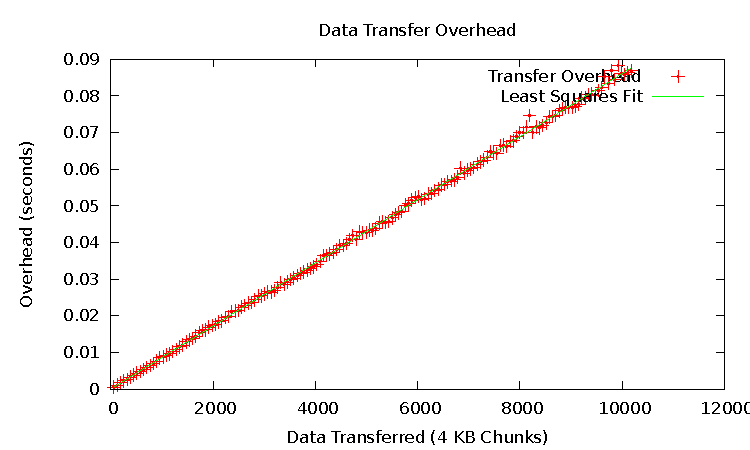
\includegraphics[scale=0.5, trim=40mm 0mm 20mm  0mm]{tachyon/dataData.pdf}
\caption{Data Transfer Overhead}
\label{tach:fig:dover}
\end{minipage}\begin{minipage}[b]{0.49\linewidth}
\centering
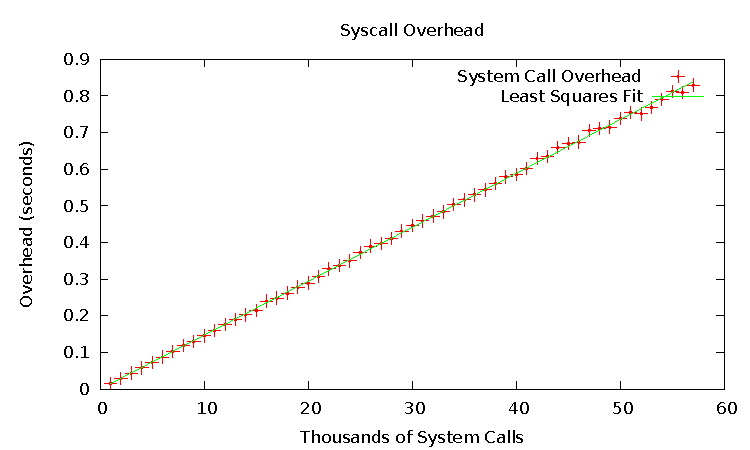
\includegraphics[scale=0.5]{tachyon/sysData.pdf}
\caption{Syscall Overhead}
\label{tach:fig:sover}
\end{minipage}
\end{figure*}

In Figure \ref{tach:fig:dover}, we see the overhead is in a linear relationship.
The overhead here is the total overhead
time for the system. While they make a difference for small data transfers, they are
rapidly dominated. This can be seen by the rapid transition to a tight grouping
around a linear relationship.


In Figure \ref{tach:fig:sover}, we again observe a nice linear relationship, showing no residual effects on performance from processing a system call. It shows that it takes less than a second of overhead to process 60,000 syscalls.

When varying the CPU load of the traced program, no noticeable difference in execution time was noticed, as we do not intercept regular computation, only system calls.

Given this, if it is known how many system calls are used, how much data is being
transferred, and how much time is being spent on the CPU, we can model how long
a given workload would take under our tracer.
\tachyon previously incurred a large number of copies and control transfers to move buffers around
in comparison with the register fetching it does for simple system calls, and
the remote memory fetch path is not optimized in the OS. However, a kernel patch
allowing for \texttt{mmap} to be used on the special file \texttt{/proc/pid/mem}
considerably ameliorate this, resulting in the new statistics above.

\paragraph{Tandem execution CPU time.}
The final source of overhead is in CPU operations.  Since \tachyon
sleeps when system calls are not being issued, it does not slow down
applications that are CPU-intensive. This is a significant advantage
over instruction-level interposition tools such as Pin~\cite{luk:2005} and
Valgrind~\cite{nethercote:2003:valgrind}, which typically suffer at least several
times overhead.

However, we are running both $\unpatched$ and $\patched$. We verified
that \tachyon can utilize independent cores to run both programs with
no additional overhead (other than the memory transfer and syscall
overhead measured above). Thus, we conclude that \tachyon can utilize
multi-core to test patches.

\paragraph{Efficiency on real programs.}

To test the efficiency of \tachyon interposition, we measured its
tandem execution against \texttt{strace} and \texttt{gdb}'s reverse
execution.  {\tt strace} is a tool built on top of \texttt{ptrace}
used to monitor system calls.  \texttt{gdb} allows programs to
back-step through operations.\footnote{We were unable to test against
  what is likely the most similar system, R2~\cite{guo:2008}, as it is
  both Windows only and requires build-time support (as well as not
  being public).} Note these tools have different goals than \tachyon;
we only use them to evaluate performance.

\texttt{gdb}'s replay mechanism derived from its reversible debugging
support. However, it proved wholly unsuitable for regions of more than
a few instructions. Due to a lack of SSE support, memcpy would be
improperly rewound and replayed. Additionally, even then the recording
overhead was more than 100x native execution, and built up a huge
memory data structure, making it impractical to benchmark.

\begin{figure}
\begin{small}
	\begin{center}
\begin{tabular}{|c|c|c|c|c|c|c|c|}
\hline
Program & Load & \tachyon  & \texttt{strace} \\
\hline \hline
\texttt{compress}  & 32M Random & 1.41  & 19.78 \\
\hline
\texttt{primegaps} & First 35 & 1.00 & 1.00 \\
\hline
\texttt{mencoder}  & h264 & 1.07 & 1.12\\
\hline
\end{tabular}
\end{center}
\end{small}
\caption{Tracing Performance (relative to native execution)}
\label{tach:fig:strace}
\end{figure}

The results compared to \texttt{strace} are shown in
Figure~\ref{tach:fig:strace}.  Overall, \tachyon was faster, sometimes by a
large margin, than a comparable syscall interposition scheme. 
This is partially because \tachyon can and does process some of its overhead while the traced program is doing work, but mostly due to the massively improved facility for retrieving remote memory via our patch to mmap /proc/pid/mem.

\paragraph{Web Server Tests.} We also tested the throughput of
\texttt{lighttpd} and \texttt{thttpd} when monitored under \tachyon.
In this test, we use ApacheBench (ab) configured to make 1000 requests
in two threads, downloading 4096 byte web page.  We ran the experiment
in two scenarios: on localhost and across the Internet.  

In the network experiment, the web servers ran at one university, and
requests were made from another university on the opposite US coast.
There was no detectable degradation for \texttt{thttpd}, and only
about a 30\% slowdown for \texttt{lighttpd}. Essentially, what this
shows is that while the system does not deal well with applications
whose progress is primarily based on the rate at which they can issue
system calls, when we move closer to a real deployment, applications
do not tend to have that as their primary limiting factor.

In the second experiment, we ran ab on localhost.  This is a
worst-case test because both web servers spin in a tight loop on a
syscall (\texttt{lighttpd} spins on \texttt{epoll}, and
\texttt{thttpd} on \texttt{poll}). 
This creates a pathological case for \tachyon, because the application
spends most of its time neither doing IO, nor doing computation, but
instead spends most of its time moving across the system call barrier.

\tachyon
took 8.9 times longer on $\texttt{lighttpd}$ (throughput decreased to
10\% of original values) and 14.2 times longer on $\texttt{thttpd}$
(throughput decreased to 7\% of original values).

To round things out, we also ran a test over a few hops on the local network.
As expected, intermediate results were measured to be between the two, with
1.17 times untraced completion to complete the test with $\texttt{thttpd}$, and 3.72
times untraced completion to complete the test with $\texttt{lighttpd}$.

With a more real network (or a more complicated webapp), we can see the
slowdown is lessened. With a real network, \texttt{epoll} will spend more
time waiting, diminishing the perceived effects.

% \texttt{mencoder} was run in a record only mode, as
% it aggressively uses all available cores, and so attempting to run two copies in
% tandem (which none of the other tracing utilities do) will necessarily produce
% massive overhead, and not truly measure the overhead of \tachyon.



%%% Local Variables: 
%%% mode: latex
%%% TeX-master: "paper"
%%% End: 

\section{Discussion}
\label{tach:sec:discussion}

\paragraph{Other Patch Testing Scenarios.} While throughout this chapter we have focused on online patch testing
where the patched version is run live, we could also run the unpatched
version live.  We note that the live program can continue executing
after a deviation, but currently the syscall sync application cannot.
Thus, by running the patched live, we are assuming that after a
deviation the right thing is to continue executing the patched
version.  However, by running the  unpatched version live, we can
check for incompatibilities while allowing for the original program to
continue executing after a deviation.

\paragraph{Honeypots.} \tachyon can also be used as a type of
lightweight honeypot. Let $\patched$ be a patch for a security
vulnerability, and $\unpatched$ be the vulnerable program. Observe
that $\patched$ and $\unpatched$ differ on exploits by definition.  By
running $\patched$ and $\unpatched$ in-tandem, \tachyon will report a
deviation on attacks.

A clever approach to running a honeypot is to run $\patched$ as the live
program, with $\unpatched$ as the sync. In this setting an attacker
only seeing the buggy program. \tachyon will report attacks, e.g., by
logging a deviation when shellcode tries to execute \texttt{/bin/sh}.
However, the system is safe from a real compromise because \tachyon
can be configured to abort execution after the deviation.



\paragraph{Debugging.} One of the most difficult to debug classes of
bugs is commonly known as heisenbugs. These are bugs which will
seemingly randomly occur or not occur with all of the inputs the
programmer knows about held constant. These traces, and the
associated replay mechanism, provide a way to step through the program
in a completely deterministic way, so that once a heisenbug has been
caught with tracing on, it has been captured and the sequence leading
to it can be carefully explored and debugged. As we capture all
inputs, this also makes it possible for the programmer to debug a
crash that took place on another machine, without having to try to
replicate the OS state to reproduce the crash.

\paragraph{Efficiency.}
Recall \tachyon uses user-land syscall interposition, and has
our approach to syscall interposition as its primary source of overhead
Currently, interposing on each system call on the live program requires 4
context switches. \tachyon context switches from $\patched$ to the
kernel, from the kernel to \tachyon, from \tachyon back to the kernel,
and finally back to $\patched$. Normal operation only has two context
switches: from user to kernel space, and back again.  A kernel-space
interposition scheme would also have only two switches. 

Recall from \S~\ref{tach:sec:eval} the overhead from copying data is almost
linear in the amount data transferred between $\patched$ and
$\unpatched$. A basic in-kernel approach would still have a linear
overhead (since data has to be copied into both virtual memory
spaces), but likely with a smaller constant factor.

Our user-land approach was chosen because it offers a clean separation
of functionality, isn't kernel dependent, and offers an easier
development environment.  Moving the system call interposition into
the kernel would not have these advantages, but would likely improve
performance. We leave further study of in-kernel tandem execution schemes
as future work.

%%% Local Variables: 
%%% mode: latex
%%% TeX-master: "paper"
%%% End: 


%Related Work
\section{Related Work}
\label{sec:related}
%  Starting blurb similar to backround blurb, surprised by this...
As this work stands at the confluence of compilation, instruction set architectures, static analysis, and type theory, there is a great deal of prior work that provided the foundation to create \bitr. There have been other attempts to perform binary type recovery. Type theorists have explored the relevant formal systems that enable us to appropriately describe the constraints imposed by the wide variety of instructions. Others have tried to build decompilers, each of which contains at least an attempt at type reconstruction.
%  Chunk related work into blobs and describe, reference to sections as you do it
\subsection{Types in Compiled Code}
In large part, previous work has considered dynamic approaches, which use execution traces to get information about concrete values. Another school of thought takes a more forensics-oriented approach, attacking the problem by looking for known data structures within a dump or trace. Finally, there is the school to which this work belongs, static type recovery, where the approach regenerates type information from a representation of the code, rather than from sample runs or matching known data structures.

\noindent {\bf Dynamic Type Description.}
Rewards~\cite{rewards} takes a dynamic, trace-oriented approach to the problem, taking execution traces and known system calls, and propagating types from system calls through the trace's reads and writes. The dynamic approach has the advantage that the analysis can know what values a memory location or register actually held at a given program point. Additionally, the dynamic approach does not have to solve the problem of indirect jumps, as when working with traces the next instruction is precisely computed. Finally, since Rewards had exact aliasing information via pointer values on each trace, flowing information from the system call barrier (their major outside source of types) is easier. While Rewards seems limited for types not present during the crossing of the system call barrier, its dynamic approach, and information from the crossing of the system call barrier could provide additional constraints to a system like \bitr\ to further improve accuracy. Howard~\cite{Slowinska2011} extends the work of Rewards by focusing on access patterns instead of simple propagation, and annotating variables from the original code, rather than locations on a dump.

\noindent {\bf Type Forensics.}
Another approach known as shape analysis~\cite{August, Haller2013a,White2013,Jung2009,Cozzie} uses dynamic traces to generate shape graphs, which they then analyze to make guesses at the types of memory locations. The systems generate the shape graph by first generating a trace, then matching the access pattern to the simplest possible graph of type structures. Some generate this trace from the compiled program, and some must annotate the program prior to compilation to achieve this trace. Once the system generates the shape graph, it compares the shape graph to multiple possibilities of what the data structure might be in attempt to classify it e.g. as a binary tree or linked list. One benefit of this technique is that when the system finds a match, more information on a name of the data structure may be available. However, if the program uses a data structure not expected by the system, some of these methods will fall short. For example, MemPick will report it to be a generic graph. It also suffers from the standard dynamic analysis issue of being unable to generate types for paths the test cases did not drive it down.

\noindent {\bf Static Type Recovery.}
Like TIE~\cite{tie}, we built \bitr\ on BAP~\cite{bap}, and also took the approach of trying to generate ranges of constraints. However, TIE performs much worse under our metric, which we feel more fully represents accuracy of more complicated types. TIE's metric is problematic for the reasons described in~\cite{sw}, but the proposed replacement metric is still dependent on a notion of distance. TIE is also slow, which hobbles its use as a large scale analysis tool. The use of DIVINE's methods was one of the bottlenecks, which we avoided in \bitr\ by recovering the type of everything that is addressable through the registers or a constant integer used along a dataflow that ended in a read or write. While the type system of TIE included structure types, TIE would rarely infer them, though its metric did not demonstrate this. Finally, if run on a static binary (e.g. without dynamic library hints), the amount TIE could infer itself was minimal.

SecondWrite~\cite{sw} instead takes the approach of lifting to a LLVM-based IR~\cite{llvm}, then using \texttt{mem2reg} to detect variables and LLVM pointer analysis to compute the types. Their reconstruction is simpler and faster than TIE's, but the approach has issues: \texttt{mem2reg} is a nice shortcut, but has the problem that \texttt{mem2reg} will not promote anything which has a use other than a load or store~\cite{llvm}. As a result, if on-stack references are in use, those stack slots will not be properly promoted to variables. Additionally, dependence on pointer analysis leaves them without a way to detect recursive types within their framework, and makes nested structures unlikely to work.

Another work focusing primarily on structure recovery~\cite{comprecon} approached the problem from the angle of figuring out what idioms compilers used to address arrays and structs, and then tried to reconstruct structs and arrays. However, by the authors' own admission, this approach cannot handle nested structs. Additionally, their dependence on assumptions about how the compiler will act and how the source language must work cause the output to be of limited use for understanding properties of code which was not necessarily built by the compilers or language expected.

\subsection{Type Theory}
Some of the inspiration for this form of type characterization \S\ref{sec:typesys} came from intersection typing~\cite{Jim1995,Shao1993}. Though we did not end up using intersection types for inferrability purposes (even the decidability of the inference turns out to be difficult and limited~\cite{interdecide}), this work informed our choice of a constraint-intersection \S\ref{sec:infmeth} approach instead of type-intersection approach.

Earlier efforts to generate typed assembly~\cite{tal,stal} also bear similarity to our work. Typed assembly language methodologies are attempting to assign types to the registers in compiled code during compilation. Some of the TAL ideas are applicable, and still others could potentially help in future reconstruction work as safer types.
However, the majority are inappropriate for the work because the compiler or author must make the code conform to the system, rather than the system describing the code.

\subsection{Decompilation}
One of the main applications for type reconstruction is decompilation. Some approaches~\cite{tydecomp} even suggest that the type reconstruction can help guide the decompilation itself rather than simply being a set of annotations applied at the end. This idea has existed~\cite{dolgova2009automatic} in decompilation for a while, but progress has been slow. More recent decompilers~\cite{phoenix} have used some of the other research~\cite{tie} in the area to improve their results as well. Given the poor state of affairs in Hex-Rays~\cite{ida}, more work in this field could improving the usability of much of the decompiler work would not be surprising.

